\documentclass[a4paper, 10pt, final, garamond]{book}
\usepackage{cours-preambule}

\titleformat{\item}{}{\arabic{item})}{.5em}{}{}
\titleformat{\subitem}{}{\arabic{item}) \alph{subitem} --}{.5em}
{}{}

\makeatletter
\renewcommand{\@chapapp}{Devoir surveill\'e -- num\'ero}
\makeatother

\begin{document}
\setcounter{chapter}{3}

\chapter{Commentaires sur le DS n\degree4}

\begin{NCprop}[width=\linewidth]{\centering\bfseries\ Rappel des malus}
    Chacune des lettres suivantes sur vos copies sont des malus de \num{1}
    point.\smallbreak
    \begin{minipage}{0.50\linewidth}
        \begin{itemize}
            \item A~: application numérique mal faite~;
            \item N~: numéro de copie incorrect ou manquant~;
            \item P~: prénom sur copies manquant~;
            \item M~: marge non laissée ou trop grande~;
            \item Q~: numéro de question mal indiqué~;
        \end{itemize}
    \end{minipage}
    \begin{minipage}{0.50\linewidth}
        \begin{itemize}
            \item C~: copie grand carreaux~;
            \item U~: unité manquante ou mauvaise~;
            \item H~: homogénéité non respectée~;
            \item S~: chiffres significatifs non respectés~;
            \item $\f$~: loi physique fondamentale brisée.
        \end{itemize}
    \end{minipage}
\end{NCprop}

\section{Commentaires généraux}

Un DS assez compliqué. Moyenne placée à \textbf{9.50/20}. Énormes variations
dans le classement~: aux extrema, 26 places gagnées et 22 places perdues.
Beaucoup de malus par rapport au dernier DS. À partir du DS05, \textbf{les malus
-C et -M seront cumulatifs}, 1 par copie concernée. Nombre de points perdus
cumulé~: \textbf{120}. 1 seule copie sans malus, plusieurs avec 6 points de
malus. Soyez critiques sur votre pratique de la science. Si c'est inhomogène,
dites-le et dans ce cas pas de malus. Si vous trouvez $k_{\rm app} < 0$ et que
ça vous choque, dites-le et il n'y aura pas de malus. Un malus -V pour
\textbf{vecteur} sera introduit au prochain DS.

\section{Exercice 1 \hfill \textcolor{red}{/26}}

\begin{enumerate}
    \item On travaille au maximum d'absorption. \hfill
        \textcolor{ForestGreen}{/2}
    \item Un catalyseur accélère une réaction sans intervenir dans l'équation
        bilan. \hfill \textcolor{ForestGreen}{/2}
    \item Il faut justifier la dégénérescence de l'ordre, la \textbf{nommer} et
        bien dire que $k_{\rm app} =
        k[\ce{H2O}]_{\fbox{0}}{}^{\alpha}[\ce{H+}]_{\fbox{0}}{}^{\beta}$. \hfill
        \textcolor{ForestGreen}{/4}
    \item Ne mettez pas des $a$ venus de nulle part en copiant le cours. Il faut
        savoir résoudre une équation différentielle linéaire d'ordre 1. \hfill
        \textcolor{ForestGreen}{/4}
    \item Il faut relier absorbance et concentration. Une régression
        \textbf{linéaire} est \textbf{linéaire}~!! Indiquez correctement ce que
        vous tracez. Indiquez les résultats de votre régression \textbf{avec les
        unités} quand il y en a (un $\ln(A)$ n'a pas d'unité). \hfill
        \textcolor{ForestGreen}{/8}
    \item Ne confondez pas le facteur pré-exponentiel avec l'absorbance. Nommez
        vos constantes intelligemment~! Si $k$ est déjà utilisé, prenez une
        autre lettre. \hfill \textcolor{ForestGreen}{/6}
\end{enumerate}

\section{Exercice 2 \hfill \textcolor{red}{/30}}

\begin{framed}
    \centering\large
    Si on vous demande d'indiquer la réponse, indiquez la réponse~: points pour
    «~réponse A~» et assimilé.
\end{framed}

\begin{minipage}{0.68\linewidth}
    \begin{enumerate}
        \item Point pour dire que les impédances étaient en série, permettant le
            PDT. \hfill \textcolor{ForestGreen}{/8}
        \item Par identification. \hfill \textcolor{ForestGreen}{/3}
        \item On simplifie directement tout avec $\w = \w_0$~! \hfill
            \textcolor{ForestGreen}{/7}
    \end{enumerate}
\end{minipage}
\hfill
\begin{minipage}{0.20\linewidth}
    \begin{enumerate}[start=4]
        \item RAS \hfill \textcolor{ForestGreen}{/6}
        \item RAS \hfill \textcolor{ForestGreen}{/4}
        \item RAS \hfill \textcolor{ForestGreen}{/2}
    \end{enumerate}
\end{minipage}


\section{Problème 1 \hfill \textcolor{red}{/63}}

\begin{minipage}{0.48\linewidth}
    \begin{enumerate}
        \item Certain-es ne doivent pas m'entendre si les fréquences audibles
            commencent à \SI{20}{kHz}… \hfill \textcolor{ForestGreen}{/2}
        \item Même baisse, même fréquence. \hfill \textcolor{ForestGreen}{/2}
        \item \textbf{Force de rappel}~: $\Ff = \pm k(\ell -\ell_0)\ex$, avec $\pm$
            selon l'orientation du ressort. Ensuite, $\ell = x_2 - x_1$. Trop de
            $x_1x_2$ qui donnent une surface, pas une longueur. \hfill
            \textcolor{ForestGreen}{/3}
        \item Sur ce DS aussi~: \textbf{système}, \textbf{référentiel},
            \textbf{bilan de toutes les forces}, \textbf{schéma}, \textbf{PDF}
            \underline{à écrire~!!} et enfin application. \hfill
            \textcolor{ForestGreen}{/11}
        \item Démontrer l'expression de $Q$ par identification. \hfill
            \textcolor{ForestGreen}{/5}
        \item RAS \hfill \textcolor{ForestGreen}{/5}
        \item On demandait explicitement le gain, pas le gain en décibels. \hfill
            \textcolor{ForestGreen}{/2}
    \end{enumerate}
\end{minipage}
\hfill
\begin{minipage}{0.48\linewidth}
    \begin{enumerate}[start=8]
        \item C'est la résonance. \hfill \textcolor{ForestGreen}{/2}
        \item Le maximum d'une fraction se trouve au minimum de son dénominateur,
            mais ici \textbf{le minimum était plus petit que 1}. Seule une personne
            l'a fait en entier et correctement. Il faut savoir étudier des fonctions
            en physique. \hfill \textcolor{ForestGreen}{/6}
        \item RAS \hfill \textcolor{ForestGreen}{/2}
        \item Points pour schéma, force sur ressort 1 et équations. \hfill
            \textcolor{ForestGreen}{/6}
        \item RAS. \hfill \textcolor{ForestGreen}{/6}
        \item Il faut savoir résoudre les équations différentielles d'ordre 2~!
            \hfill \textcolor{ForestGreen}{/9}
        \item RAS. \hfill \textcolor{ForestGreen}{/2}
    \end{enumerate}
\end{minipage}

\section{Problème 2 \hfill \textcolor{red}{/54}}

\begin{minipage}{0.48\linewidth}
    \begin{enumerate}
        \item RAS. \hfill \textcolor{ForestGreen}{/3}
        \item Il faut faire l'étude en entier, justifier chaque étape de la
            réflexion. \hfill \textcolor{ForestGreen}{/9}
        \item Simple association~: série puis parallèle. \hfill
            \textcolor{ForestGreen}{/3}
        \item Beaucoup de mélange ici~: une impédance faible en parallèle d'une
            impédance élevée est équivalente à l'impédance faible. \hfill
            \textcolor{ForestGreen}{/3}
        \item Double pont diviseur comme discuté en soutien et intégralement corrigé
            3 fois dans le TD. \hfill \textcolor{ForestGreen}{/7}
    \end{enumerate}
\end{minipage}
\hfill
\begin{minipage}{0.48\linewidth}
    \begin{enumerate}
        \item Étude asymptotique~: impasse totale. Dommage. \hfill
            \textcolor{ForestGreen}{/10}
        \item Attention à bien calculer les modules. \hfill
            \textcolor{ForestGreen}{/2}
        \item Utilisez $G_{\dB}(\w_r) = G_{\dB, \max} - \SI{3}{dB}$. \hfill
            \textcolor{ForestGreen}{/3}
        \item 1 personne arrivée au bout. RAS. \hfill \textcolor{ForestGreen}{/5}
        \item Il vaut mieux isoler par l'extérieur. \hfill
            \textcolor{ForestGreen}{/5}
        \item RAS. Justifiez le quart de période. \hfill \textcolor{ForestGreen}{/4}
    \end{enumerate}
\end{minipage}

\section{Problème 3 \hfill \textcolor{red}{/30}}

\begin{enumerate}
    \item Dire «~comme montré problème 2~» n'est pas une justification valable.
        Les problèmes sont indépendants. Il était attendu de faire l'étude
        complète des filtres. Dommage pour les quelques personnes ayant inversé
        interrupteur ouvert et fil… \hfill \textcolor{ForestGreen}{/16}
    \item Hécatombe. \hfill \textcolor{ForestGreen}{/14}
\end{enumerate}

\vfill

\begin{center}
    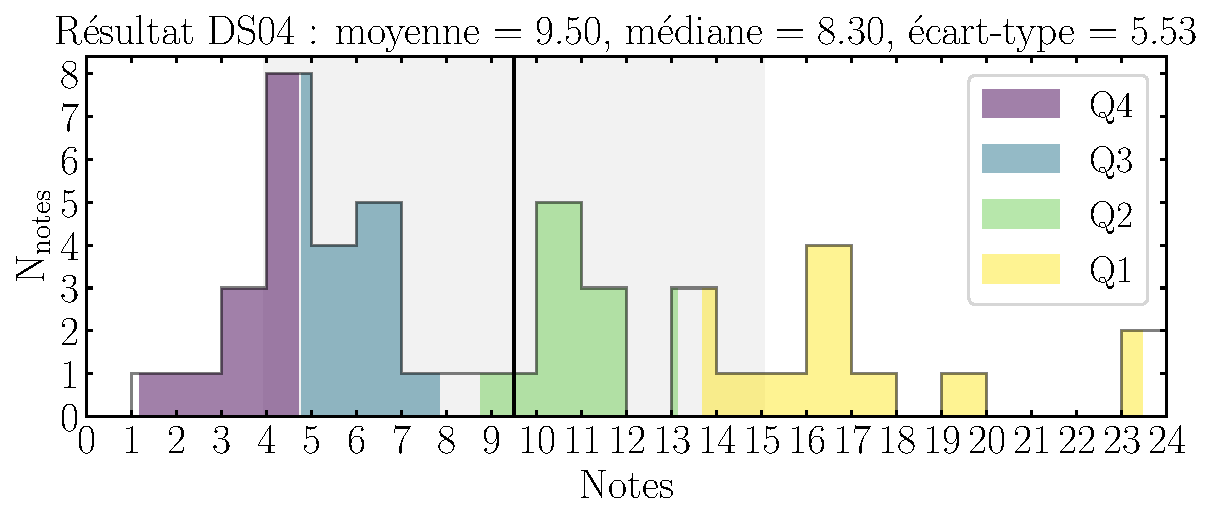
\includegraphics[width=.72\linewidth]{res_DS04.pdf}
\end{center}

\vfill

\end{document}
